\documentclass[a4paper]{article}

\usepackage[english]{babel}
\usepackage[utf8]{inputenc}
\usepackage{amsmath}
\usepackage{graphicx}
\usepackage[colorinlistoftodos]{todonotes}
\usepackage{tikz}
\usetikzlibrary{fit,positioning}
\usepackage{authblk}
\usepackage{natbib}
\usepackage[algo2e]{algorithm2e}
\usepackage{algorithmic}  
\usepackage{algorithm}
\usepackage{comment}
\title{Joint Modeling of Content-Partitioned Multinetwork Embeddings (CPME) and Point Process Approach}
\author{Bomin Kim}

\begin{document}
\maketitle
\section{Ideas}
Current CPME model does not involve any of temporal component, which plays a key role in email interactions. Intuitively, past interaction behaviors significantly influence future ones; for example, if an actor $i$ sent an email to actor $j$, then $j$ is highly likely to send an email back to $i$ as a response (i.e. reciprocity). Moreover, the recency and frequency of past interactions can also be considered to effectively predict future interactions. Thus, as an exploratory data analysis, point process model for directional interaction is applied to the North Carolina email data. Starting from the existing framework focused on the analysis of content-partitioned subnetworks, I would suggest an extended approach to analyze the data using the timestamps in the email, aiming to develop a joint dynamic or longitudinal model of text-valued ties.\\ \newline
 CPME model is a Bayesian framework using two well-known methods: Latent Dirichlet Allocation (LDA) and Latent Space Model (LSM). Basically, existence of edge depends on topic assignment $k$ (LDA) and its corresponding interaction pattern c. Each topic $k=1,…,K$ has one interaction pattern c=1,…,C, and each interaction pattern posits unique latent space (LSM), thus generating $A\times A$ matrix of probabilities $P^{(c)}$ that a message author
a will include recipient $r$ on the message, given that it is about
a topic in cluster $c$.  Incorporating point process approach, now assume that under each interaction pattern, we have $A\times A$ matrix of stochastic intensities at time $t$, $\lambda^{(c)}(t)$, which depend on the history of interaction between the sender and receiver. 
\newpage
\section{CPME + Point Process Model}
In this section, we introduce multiplicative Cox regression model for the edge formation process in a longitudinal communication network. For concreteness, we frame our discussion of this model in terms of email data, although it is generally applicable to any similarly-structured communication data.
\subsection{Point Process Framework}
A single email, indexed by $d$, is represented by a set of tokens $w^{(d)} = \{w^{(d)}_m \}_{m=1}^{M^{(d)}}$ that comprise the
text of that email, an integer $i^{(d)} \in \{1,...,A\}$ indicating the identity of that email’s sender, an integer $j^{(d)} \in \{1,...,A\}$ indicating the identity of that email’s receiver, and an integer $t^{(d)} \in [0, T]$ indicating the (unix time-based) timestamp of that email. To capture the relationship between the interaction patterns expressed in an email and that email’s recipients, documents that share the interaction pattern $c$ are associated with an $A\times A$ matrix of $N^{(c)}_{ij}(t)$, a counting process denoting the number of edges (emails) of interaction pattern $c$, from actor $i$ to actor $j$ up to time $t$. NOTE: We use the partition $c$ since we expect that some interaction patterns have little variation among the pairs of actors (e.g. broadcasting), while some have large variation (e.g. meeting scheduling, personal affairs). \\ \newline Combining the individual counting processes of all potential edges,  $\mathbf{N}^{(c)}(t)$ is the multivariate counting process with $\mathbf{N}^{(c)}(t)=(N^{(c)}_{ij}(t): i, j \in {1, ..., A}, i \neq j)$. Here we make no assumption about the independence of individual edge counting process. As in \cite{Vu2011}, we model the multivariate counting process via Doob-Meyer decomposition:
\begin{equation}
\mathbf{N}^{(c)}(t)=\int_0^t\boldsymbol{\lambda}^{(c)}(s)ds + \mathbf{M}(t)
\end{equation}
where essentially $\boldsymbol{\lambda}^{(c)}(t)$ and $\mathbf{M}(t)$ may be viewed as the (deterministic) signal and (martingale) noise, respectively.\\ \newline
Following the multiplicative Cox model of the intensity process $\boldsymbol{\lambda}^{(c)}(t)$ given $\boldsymbol{H}^{(c)}_{t-}$, the entire past of the network related to the interaction pattern $c$ up to but not including time $t$, we consider for each potential directed edge $(i, j)$ the intensity forms:
\begin{equation}
\lambda^{(c)}_{ij}(t|\boldsymbol{H}^{(c)}_{t-})=\lambda^{(c)}_0(t)\cdot \mbox{exp}(\boldsymbol{\beta}^{(c)T}\boldsymbol{x}^{(c)}(i, j, t))\cdot 1\{j \in \mathcal{J}^{(c)}_{(i, t)}\}
\end{equation}
where $\lambda_0^{(c)}(t)$ is the baseline hazards for the interaction pattern $C$, $\boldsymbol{\beta}^{(c)}$ is an unknown vector of coefficients in $\boldsymbol{R}^{p}$, $\boldsymbol{x}^{(c)}(i, j, t)$ is a vector of $p$ statistics for directed edge $(i, j)$ constructed based on
$\boldsymbol{H}^{(c)}_{t-}$, and $\mathcal{J}^{(c)}_{(i, t)}$ is the predictable receiver set of sender $i$ at time $t$ within all actors $A^{(c)}$. NOTE: We assume that all possible actor set $A^{(c)}$ varies depending on the interaction pattern (e.g. confidential communication do not move outside of certain actors).
\subsection{Generative Process}
The generative process of this model follows that of \cite{Blei2003} and \cite{rosen2004author}. Same as LDA, documents are represented as random mixtures over latent topics, where each topic is characterized by a distribution over words. However, one difference is that each documents is connected to one interaction pattern, and the topic distributions vary depending on the interaction pattern. Following is the generative process for each document in a corpus $D$:
\begin{itemize}
	\item[1.] {Choose $\phi^{(k)} \sim \mbox{Dir}(\delta, \bf n)$}\\
	- A “topic” $k$ is characterized by a discrete distribution over $V$ word types with probability vector $\phi^{(k)}$. A symmetric Dirichlet prior with concentration parameter $\delta$ is placed \textbf{[See Algorithm 1]}.
\item[2.] For each of the $C$ interaction patterns \textbf{[See Algorithm 2]}:
\begin{itemize}
	\item[(a)] Choose $\boldsymbol{\theta}^{(c)}\sim \mbox{Dir}(\alpha, \bf m)$\\
- As an extension of LDA, each email, indexed by $d$, has a discrete distribution over topics $\boldsymbol{\theta}^{(c)}$. A Dirichlet prior
with concentration parameter $\alpha$ is placed.
\item[(b)] Choose $\boldsymbol{\beta}^{(c)}\sim \mbox{Normal}(\textbf{0}, \sigma^2I_P)$\\ 
- $\mbox{Normal}(\textbf{0}, \sigma^2I_P)$ is just one example.
\end{itemize}
\item[3.] For each of the $D$ documents \textbf{[See Algorithm 3]}:
\begin{itemize}
	\item[(a)] Choose $c^{(d)}\sim \mbox{Multinomial}(\gamma)$\\
	- Each document $d$ is associated with one ``interaction pattern" among $C$ different types, with parameter $\gamma$.
	\item[(b)] Choose $\boldsymbol{N}^{(c^{(d)})}(t) \sim \mbox{CP}(\boldsymbol{\lambda}^{(c^{(d)})}(t))$\\
	- The actual update of the counting process $N^{(c)}_{ij}(t)$ of the email $d$ will be  $N^{(c^{(d)})}_{i^{(d)}j^{(d)}}(t^{(d)})=N^{(c^{(d)})}_{i^{(d)}j^{(d)}}(t^{(d)}-)+1$. This one increment of $N^{(c)}_{ij}(t)$ is related to $\bar{M}^{(d)}$ tokens, which will be used for the next algorithm.
\end{itemize}
\item[4.] For each of the $M$ words \textbf{[See Algorithm 4]}:
\begin{itemize}
	\item[(a)] $z_m^{(d)} \sim \mbox{Multinomial}(\boldsymbol{\theta}^{(c)})$\\ 
- In this case, we use interaction-based $\boldsymbol{\theta}^{(c)}$, unlike CPME.
\item[(b)] $w_m^{(d)} \sim\mbox{Multinomial} (\phi^{(z_m^{(d)})})$
\end{itemize}
\end{itemize} 
 \begin{algorithm}[H]
 	\SetAlgoLined
 	\caption{Topic Word Distributions}
 	\For{k=1 to K}{
 		draw $\phi^{(k)}$ $\sim$ Dir($\delta, \bf n$)
 	}
 \end{algorithm}
 \begin{algorithm}[H]
 	\SetAlgoLined
 	\caption{Interaction Patterns}
 	\For{c=1 to C}{
 		draw $\boldsymbol{\theta}^{(c)}$ $\sim$ Dir($\alpha, \bf m$)\\
 		draw $\boldsymbol{\beta}^{(c)}\sim \mbox{Normal}(\textbf{0}, \sigma^2I_P)$\\
 	\For{i=1 to A}{
 	\For{j=1 to A}{
 		\If{i $\neq$ j}{ set $\lambda^{(c)}_{ij}(t)=\lambda^{(c)}_0(t)\cdot \mbox{exp}(\boldsymbol{\beta}^{(c)T}\boldsymbol{x}^{(c)}(i, j, t))\cdot 1\{j \in \mathcal{J}^{(c)}_{(i, t)}\}$ }
 	\Else {set $\lambda^{(c)}_{ij}(t)=0$}
 	\textcolor{red}{Q: Do we need to estimate $\lambda^{(c)}_0(t)$? How? Maybe can have one common parameter $\lambda$ and sample $c$ different baseline intensities.  }
 		}}
 	}
 \end{algorithm}
 \begin{algorithm}[H]
 	\SetAlgoLined
 	\caption{Document-Interaction Pattern Assginments}
 	\For{d=1 to D}{
 		draw $c^{(d)}$ $\sim$ Multinomial($\gamma$)\\
 			draw $\boldsymbol{N}^{(c^{(d)})}(t) \sim \mbox{CP}(\boldsymbol{\lambda}^{(c^{(d)})}(t))$
 	}
 \end{algorithm}
 \begin{algorithm}[H]
 	\SetAlgoLined
 	\caption{Tokens}
 	\For{d=1 to $D$}{
 		set $\bar{M}^{(d)}=\mbox{max}(1,{M}^{(d)})$\\
 		\For{m=1 to $\bar{M}^{(d)}$}{
 			draw $z_m^{(d)} \sim \mbox{Multinomial}(\boldsymbol{\theta}^{(c)})$\\
 			\If{${M}^{(d)}\neq 0$}{draw $w_m^{(d)} \sim\mbox{Multinomial} (\phi^{(z_m^{(d)})})$
 				} }
}
 \end{algorithm}
 	\textcolor{red}{Q: As in CPME, the topic assignments $z_m^{(d)}$ should have some connection to $N_{ij}^{(c)}(t)$ (the topics used in the document affects the number of emails between $i$ and $j$). How? Currently the plate notation in Figure 1 has the arrow, but in the generative process it isn't. Or, is it fine to delete the arrow and use the current generative process?}
 \small
 \begin{figure}[ht]
 	\centering
 	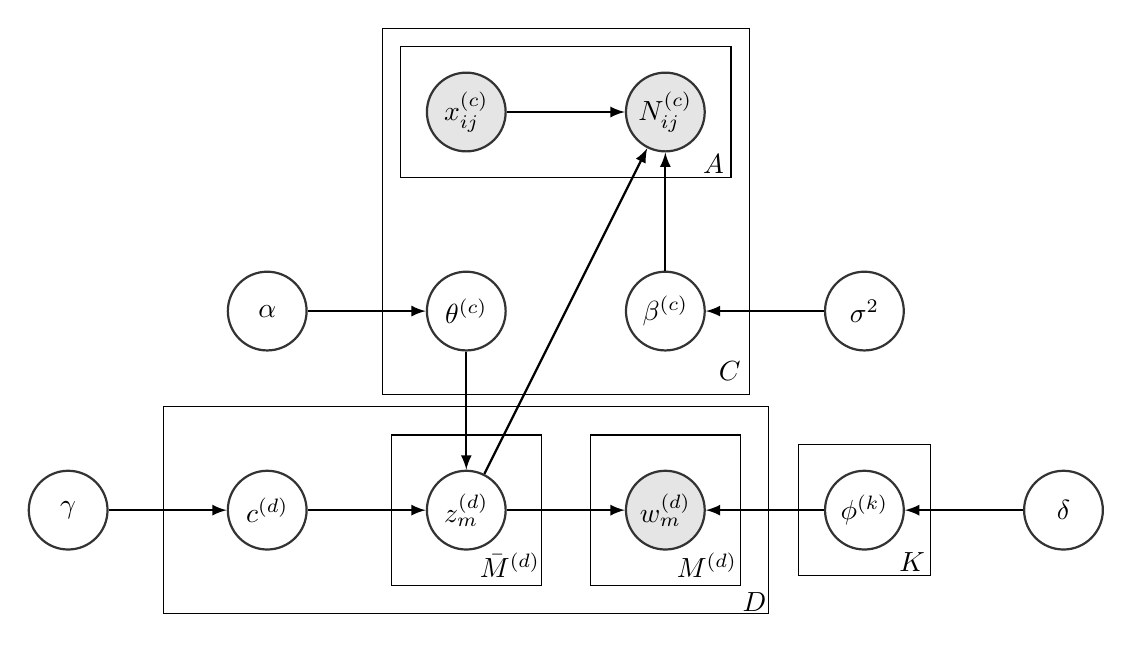
\begin{tikzpicture}
 	\tikzstyle{main}=[circle, minimum size = 10mm, thick, draw =black!80, node distance = 15mm]
 	\tikzstyle{connect}=[-latex, thick]
 	\tikzstyle{box}=[rectangle, draw=black!100]
 	\node[main, fill = white!100] (gamma) [label=center:$\gamma$] { };
 	\node[main] (c) [right=of gamma,label=center:$c^{(d)}$] { };
 	\node[main] (z) [right=of c,label=center:$z_m^{(d)}$] {};
 	\node[main, fill = black!10] (w) [right=of z,label=center:$w_m^{(d)}$] { };
 		\node[main] (theta) [above=of z,label=center:$\theta^{(c)}$] { };
 		 	\node[main] (alpha) [left=of theta,label=center:$\alpha$] { };
 	\node[main] (phi) [right=of w,label=center:$\phi^{(k)}$] { };
 	\node[main] (delta) [right=of phi,label=center:$\delta$] { };
 	 	\node[main] (beta) [above=of w,label=center:$\beta^{(c)}$] { };
 	 		\node[main, fill = black!10] (x) [above=of theta,label=center:$x_{ij}^{(c)}$] { };
 	 			\node[main, fill = black!10] (N) [above=of beta,label=center:$N_{ij}^{(c)}$] { };
 	 		\node[main] (sigma) [right=of beta,label=center:$\sigma^2$] { };
 	\path (gamma) edge [connect] (c)
 	(c) edge [connect] (z)
 	(z) edge [connect] (w)
 	(theta) edge [connect] (z)
 	(alpha) edge [connect] (theta)
 	(phi) edge [connect] (w)
 	(delta) edge [connect] (phi)
 	(sigma) edge [connect] (beta)
 	(x) edge [connect] (N)
 	(beta) edge [connect] (N)
 	(z) edge [connect] (N);
 	\node[rectangle, inner sep=5.5mm, draw=black!100, fit= (theta) (beta) (x) (N)] {};
 		\node[rectangle, inner sep=0mm, fit=  (theta) (beta),label=below right:$C$, xshift=13mm, yshift=0mm] {};
 			\node[rectangle, inner sep=0mm, fit=  (x) (N),label=below right:$A$, xshift=11mm, yshift=1mm] {};
 	\node[rectangle, inner sep=3.2mm, draw=black!100, fit= (phi)] {};
 		\node[rectangle, inner sep=3.2mm, draw=black!100, fit= (x) (N)] {};
 		\node[rectangle, inner sep=0mm, fit= (phi),label=below right:$K$, xshift=-2mm, yshift=1mm] {};
 	\node[rectangle, inner sep=0mm, fit= (w),label=below right:$M^{(d)}$, xshift=-5mm, yshift=1mm] {};
 		\node[rectangle, inner sep=0mm, fit= (w),label=below right:$\bar{M}^{(d)}$, xshift=-30mm, yshift=1mm] {};
 	\node[rectangle, inner sep=4.4mm,draw=black!100, fit= (w)] {};
 		\node[rectangle, inner sep=4.4mm,draw=black!100, fit= (z)] {};
 	\node[rectangle, inner sep=4mm, fit= (z) (w),label=below right:$D$, xshift=12mm] {};
 	\node[rectangle, inner sep=8mm, draw=black!100, fit = (c) (z) (w)] {};
 	\end{tikzpicture}
 	\caption{Plate notation of the CPME+Point process model}
 	\label{fig:plate}
 \end{figure}
 \normalsize
\subsection{Dynamic covariates to measure network effects}
The network statistics $x^{(c)}(i, j, t)$ of equations (2), corresponding to the ordered pair $(i, j)$, can be time-invariant (such as gender) or time-dependent (such as the number of two-paths from $i$ to $j$ just before time $t$). Since time-invariant covariates can be easily specified in various manners (e. g. homophily or group-level effects), here we only consider specification of dynamic covariates.\\ \newline
Following \cite{PerryWolfe2012}, we use 6 effects as components of $x^{(c)}(i, j, t)$. The first two behaviors (send and receive) are dyadic, involving exactly two actors,
while the last four (2-send, 2-receive, sibling, and cosibling) are triadic, involving exactly three actors. However, different from \cite{PerryWolfe2012}, we define the effects not based on finite sub-interval, which require large number of dimention. Instead, we create single statistic for each effect by incorporating the recency of event into the statistic itself. Moreover, we take the interaction pattern $c$ into account as well, based on the topic-token-interaction pattern assignment from LDA. \\ \newline 
1. $\textbf{send}^{(c)}(a, r, t)=\sum\limits_{d: t_d<t} \frac{\bar N^{(c|d)}}{\bar N^{(d)}}\cdot I\{a\rightarrow r\}\cdot g(t-t_d)$\\
2. $\textbf{receive}^{(c)}(a, r, t)=\sum\limits_{d: t_d<t} \frac{\bar N^{(c|d)}}{\bar N^{(d)}}\cdot I\{r\rightarrow a\}\cdot g(t-t_d)$\\
3. $\textbf{2-send}^{(c)}(a, r, t)=\sum\limits_{h \neq a, r}\Large(\sum\limits_{d: t_d<t} \frac{\bar N^{(c|d)}}{\bar N^{(d)}}\cdot I\{a\rightarrow h\}\cdot g(t-t_d)\Large)\Large(\sum\limits_{d: t_d<t} \frac{\bar N^{(c|d)}}{\bar N^{(d)}}\cdot I\{h\rightarrow r\}\cdot g(t-t_d)\Large)$\\
4. $\textbf{2-receive}^{(c)}(a, r, t)=\sum\limits_{h \neq a, r}\Large(\sum\limits_{d: t_d<t} \frac{\bar N^{(c|d)}}{\bar N^{(d)}}\cdot I\{h\rightarrow a\}\cdot g(t-t_d)\Large)\Large(\sum\limits_{d: t_d<t} \frac{\bar N^{(c|d)}}{\bar N^{(d)}}\cdot I\{r\rightarrow h\}\cdot g(t-t_d)\Large)$\\
5. $\textbf{sibling}^{(c)}(a, r, t)=\sum\limits_{h \neq a, r}\Large(\sum\limits_{d: t_d<t} \frac{\bar N^{(c|d)}}{\bar N^{(d)}}\cdot I\{h\rightarrow a\}\cdot g(t-t_d)\Large)\Large(\sum\limits_{d: t_d<t} \frac{\bar N^{(c|d)}}{\bar N^{(d)}}\cdot I\{h\rightarrow r\}\cdot g(t-t_d)\Large)$\\
6. $\textbf{cosibling}^{(c)}(a, r, t)=\sum\limits_{h \neq a, r}\Large(\sum\limits_{d: t_d<t} \frac{\bar N^{(c|d)}}{\bar N^{(d)}}\cdot I\{a\rightarrow h\}\cdot g(t-t_d)\Large)\Large(\sum\limits_{d: t_d<t} \frac{\bar N^{(c|d)}}{\bar N^{(d)}}\cdot I\{r\rightarrow h\}\cdot g(t-t_d)\Large)$\\\newline
Here, $g(t-t_d)$ reflects the difference between current time $t$ and the timestamp of previous email $t_d$, thus measuring the recency. Inspired by the self-exciting Hawkes process, which is often used to model the temporal effect of email data, we can take the exponential kernel $g(t-t_d)=we^{-w(t-t_d)}$ where $w$ is the parameter of speed at
which sender replies to emails, with larger values indicating faster response times. Indeed, $w^{-1}$ is the expected number of hours it takes to reply to a typical email.
\subsection{Inference}
First of all, we figure out how to obtain the 6 covariates in $x^{(c)}(a, r, t)$ defined in the previous section. Notice that one special thing about this approach is that for each term we put weights in front of typical network statistics, that is, $$\frac{\bar N^{(c|d)}}{\bar N^{(d)}}.$$
Similar to the generative process of CPME, define $$\bar N^{(d)}=\mbox{max}(1, N^{(d)})\quad\mbox{and}\quad \bar N^{(c|d)}=\sum_{n=1}^{\bar N^{(d)}}\delta(l_{z_n^{(d)}}=c).$$
In order to obtain $\bar N^{(c|d)}$, we need the probability that a token is assgined to a particular topic related to specific interaction pattern conditional on the topic assignments of all other tokens, the word-types of all other tokens, and hyper-parameters. Since we use uniform distribution for topic-interaction pattern assignments (i.e. $l_t \sim \mbox{Unif}(1, C)$), 
$$P(l_{z_n^{(d)}}=c|\mathcal{W}, \mathcal{Z}_{\backslash d, n}, \beta, \boldsymbol{n}, \alpha, \boldsymbol{m})=\sum\limits_{t:l_t=c}P({z_n^{(d)}}=t | \mathcal{W}, \mathcal{Z}_{\backslash d, n}, \beta, \boldsymbol{n}, \alpha, \boldsymbol{m}).$$ 
Now following the existing derivation from the work of Matthew Denny, by applying Bayes rule, we get $$\sum\limits_{t:l_t=c}P({z_n^{(d)}}=t | \mathcal{W}, \mathcal{Z}_{\backslash d, n}, \beta, \boldsymbol{n}, \alpha, \boldsymbol{m})=\sum\limits_{t:l_t=c}P({z_n^{(d)}}=t, w_n^{(d)} | \mathcal{W}_{\backslash d, n}, \mathcal{Z}_{\backslash d, n}, \beta, \boldsymbol{n}, \alpha, \boldsymbol{m})$$
$$\quad\quad\quad\quad\quad\quad\quad\quad\quad\quad\quad\quad=\sum\limits_{t:l_t=c} \frac{N_{\backslash d, n}^{(t|d)}+\alpha m_t}{N^{d}-1+\alpha}\cdot \frac{N_{\backslash d, n}^{(w_n^{(d)}|t)}+\beta n_v}{N_{\backslash d, n}^{(t)}+\beta} $$\\\newline
After we fully construct the matrix of covariates $x^{(c)}(a, r, t)$, we move to estimation steps. Assuming each interaction has a single receiver (no multicast), we model the stochastic intensity of the multivariate counting process $N$ as \begin{equation}\lambda_t(i,j)=\bar\lambda_t(i)\cdot \mbox{exp}\{\beta^Tx_t(i, j)\}\cdot 1\{j \in \mathcal{J}_t(i)\},
\end{equation} 
where $\beta$ is an unknown vector of coefficients in $\boldsymbol{R}^{p}$. After treating the baseline rate $\bar\lambda_t(i)$ as a nuisance parameter, estimation for $\beta$ proceeds by maximizing the so-called partial likelihood of \cite{cox1992regression}: 
\begin{equation}
PL_t(\beta)=\prod_{t_m\leq t} \frac{\mbox{exp}(\beta^Tx_{t_m}(i_m, j_m))}{\sum_{j\in \mathcal{J}_{t_m}(i_m)} \mbox{exp}(\beta^Tx_{t_m}(i_m, j))},
\end{equation}
where $t_m$, $i_m$, and $j_m$ are the time, sender, and receiver
of the $m$th event.
Further, we can estimate the coefficient vector $\beta$ using the log-partial likelihood at time $t$:
\begin{equation}
\mbox{log}PL_t(\beta)=\sum_{t_m\leq t} \Big\{\beta^Tx_{t_m}(i_m, j_m)-\mbox{log}\big[\sum_{j\in \mathcal{J}_{t_m}(i_m)} \mbox{exp}\{\beta^Tx_{t_m}(i_m, j)\}\big]\Big\}.
\end{equation}
The function $\mbox{log}PL_t(\cdot)$ is concave, so it can be maximized using the first two derivatives, the gradient $U_t(\beta)=\bigtriangledown[\mbox{log}PL_t(\beta)]$ and negative Hessian $I_t(\beta)=-\bigtriangledown^2[\mbox{log}PL_t(\beta)]$ via the Newton-Raphson algorithm. See \cite{PerryWolfe2012} for the details.\\\\
The model can be extended for interactions that possibly involve a single sender and multiple receivers such as emails, which we call a multicast interaction. Let the tuple $(t, i, J)$ indicate that at time $t$, sender $i$ interacted with receiver set $J$. In addition, let $|J|$ denote the cardinality of the receiver set $J$. Then, we can write the modified version of (3) and (5) as below:
\begin{equation}\lambda_t(i,J)=\bar\lambda_t(i; |J|)\cdot \mbox{exp}\{\sum_{j\in J}\beta_0^Tx_t(i, j)\}\cdot\prod_{j\in J} 1\{j \in \mathcal{J}_t(i)\},
\end{equation}
\begin{equation}
\mbox{log}PL_t(\beta)=\sum_{t_m\leq t} \Big\{\sum_{j\in J_m}\beta^Tx_{t_m}(i_m, j)-\mbox{log}\big[\sum_{\substack{j\subseteq \mathcal{J}_{t_m}(i_m)\\|J|=|J_m|}}\mbox{exp}\{\sum_{j\in  J}\beta^Tx_{t_m}(i_m, j)\}\big]\Big\}.
\end{equation}
Fitting the model above is quite complicated due to the double sums. Thus, instead of using the multicast model, we can use the alternative, the approximate partial loglikelihood, which is obtained by treating the multicast interaction as multiple pairwise interactions. For instance, an email with the tuple $(t, i, J=(j_1, j_2))$ is treated as two separate emails $(t, i, j_1)$ and $(t, i, j_2)$. Under this transformation, the obtained approximate partial loglikelihood is:\begin{equation}
\mbox{log}\widetilde{PL}_t(\beta)=\sum_{t_m\leq t} \Big\{\sum_{j\in J_m}\beta^Tx_{t_m}(i_m, j)-|J_m|\mbox{log}\big[\sum_{j\subseteq \mathcal{J}_{t_m}(i_m)}\mbox{exp}\{\beta^Tx_{t_m}(i_m, j)\}\big]\Big\}
\end{equation}
and $\mbox{log}PL_t(\beta)\approx \mbox{log}\widetilde{PL}_t(\beta)$. To fit the model in a simpler way, we use (8) when estimating the coefficitients $\beta$. For implementation and simulation processes in detail, see \cite{PerryWolfe2012}.  This framework can be viewed as one version of relational event model \cite{Butts2008}, accounting for repeated directed actions and multicast inteactions. Therefore, the coefficients measuring the common effects such as homophily or transitivity can be interpreted in the same context as in \cite{Butts2008}.
\section{Preliminary Analysis}
Hurricane Sandy was the most destructive hurricane in 2012, which hit North Carolina on late October (October 28, Governor Bev Perdue declared a state of emergency in 24 western counties due to snow and strong winds). In our dataset, there are three counties which cover the date of Hurricane Sandy (October 22, 2012 – November 2, 2012), so we focus on the three counties, since the timestamp of email in this case is much more important than usual case without any disastrous event.
\subsection{Dare County}
\footnotesize
\begin{table}[ht]
	\centering
	\begin{tabular}{ |c|ccc|c| } 
		\hline 
		\textbf{Period} &\textbf{Before Sandy} & \textbf{During Sandy} & \textbf{After Sandy} & \textbf{Overall} \\ 	\hline
			\textbf{\# emails}& 1933 & 1563 & 1467 & 4963 \\ 
		\hline
	\end{tabular}
	\caption{ Summary of Dare county email data based on time period}
	\label{table:nullDare2}
\end{table}
\normalsize
Before Sandy ranges from 2012-09-01 to 2012-10-21 (7 weeks), During Sandy ranges from 2012-10-22 to 2012-11-02 (2 weeks), and After Sandy ranges from 2012-11-03 to 2012-11-30 (4 weeks).
\footnotesize
\begin{figure}[ht]
	\centering
	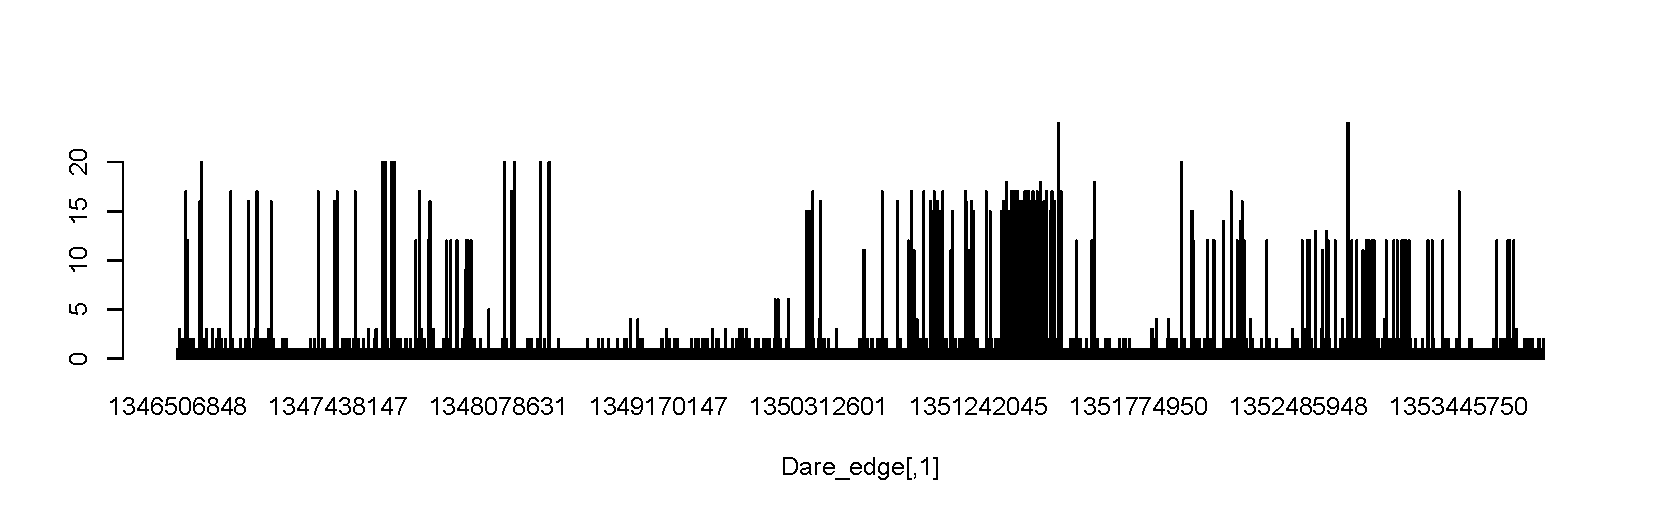
\includegraphics[width=1.1\textwidth]{DareEmails.pdf} 
	\caption{Frequency of Dare county emails from 2012-09-01 to 2012-11-30  }
	\label{fig:Emailplots}
\end{figure}
\begin{table}[ht]
	\centering
	\begin{tabular}{ |c|cc| } 
		\hline 
		\textbf{Time Interval} &\textbf{send} & \textbf{receive} \\ 	
		\hline  $[-\infty, t)$&  2.128, 2.659, 2.355, 2.919& 0.292, 0.257, 0.047, 0.110\\  $[t-30 m, t)$ &  0.262, -0.064, 0.782, 0.317 &2.087, 1.287 , 2.346, 1.870\\  $[t-2h, t-30m)$& 0.383, 0.157 , 0.024, -0.045 &0.553, 0.082, 0.794, 0.269\\ $[t-8h, t-2h)$ & 0.816, 0.054 , 0.077, 0.381 &-0.221, 0.048, 0.298, -0.012 \\ $[t-32h, t-8h)$& 0.085, 0.014,  0.228, 0.070 &0.101, 0.017, -0.033, 0.019\\ $[t-5.33d, t-32h)$&  0.103, 0.025, 0.092, 0.008 &-0.027, -0.016, -0.033, -0.009 \\ $[t-21.33d, t-5.33d)$  & 0.052, 0.000, 0.059, 0.010& 0.013, 0.030 , -0.016, 0.013\\ 
		$[-\infty, t-21.33d)$  & 0.052, 0.103, 0.027, 0.021  & 0.008, 0.000, 0.020, -0.005\\
		\hline
	\end{tabular}
	\caption {Estimated coefficients and approximate standard errors for dyadic effects of Dare county data (before Sandy, during Sandy, after Sandy, overall)}
	\label{table:nullDare}
\end{table}
\footnotesize
\begin{figure}[ht]
	\centering
	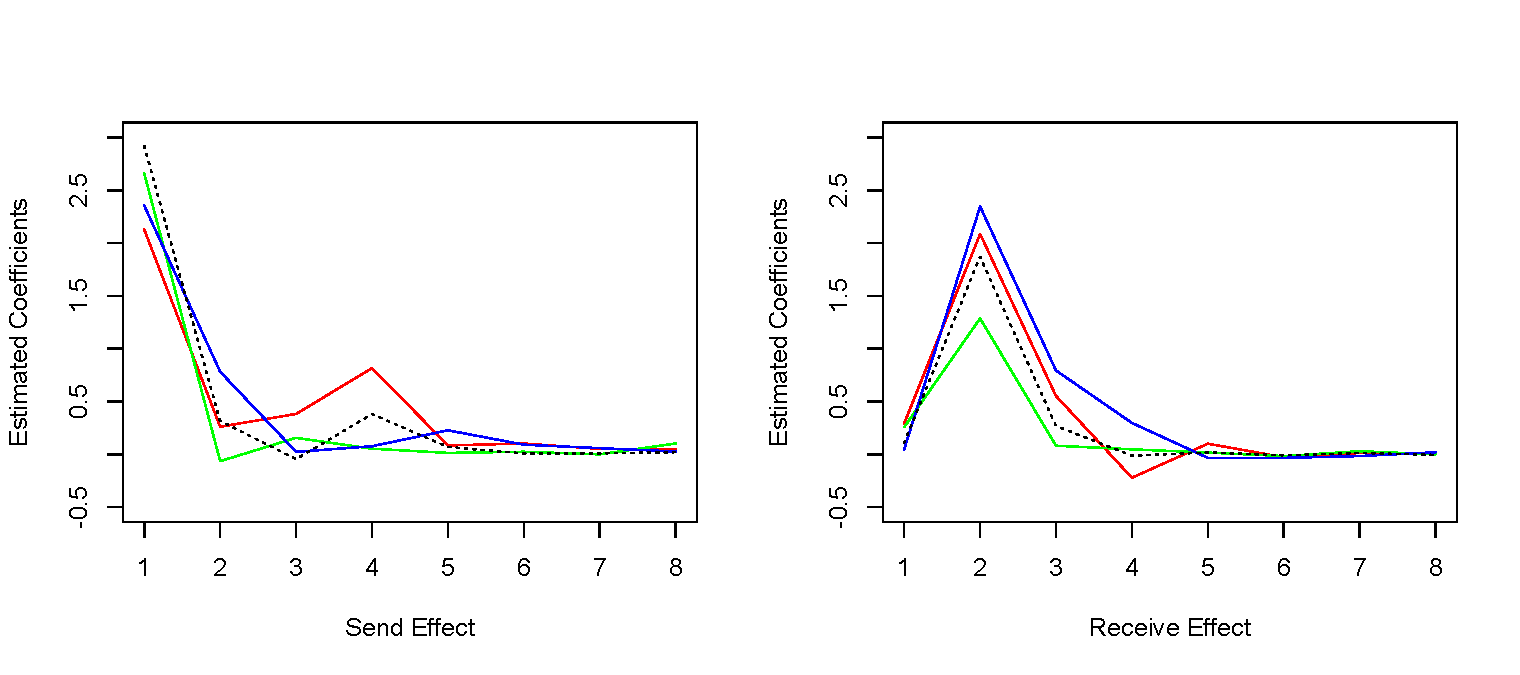
\includegraphics[width=1.1\textwidth]{Dareplot.pdf} 
	\caption{Comparison of Send (left) and Receive (right) effect based on periods in Table 1. (Red=Before, Green=During, Blue=After, and dot=Overall)}	\label{fig:Emailplo22t}
\end{figure}
\subsection{Lenoir County}
\footnotesize
\begin{table}[ht]
	\centering
	\begin{tabular}{ |c|ccc|c| } 
		\hline 
		\textbf{Period} &\textbf{Before Sandy} & \textbf{During Sandy} & \textbf{After Sandy} & \textbf{Overall} \\ 	\hline
		\textbf{\# emails}& 216 & 83 & 302 & 601 \\ 
		\hline
	\end{tabular}
	\caption{ Summary of Lenoir county email data based on time period}
	\label{table:nullDare22}
\end{table}
\normalsize
Before Sandy ranges from 2012-10-01 to 2012-10-21 (3 weeks), During Sandy ranges from 2012-10-22 to 2012-11-02 (2 weeks), and After Sandy ranges from 2012-11-03 to 2012-12-31 (8 weeks).
\footnotesize
\begin{figure}[ht]
	\centering
	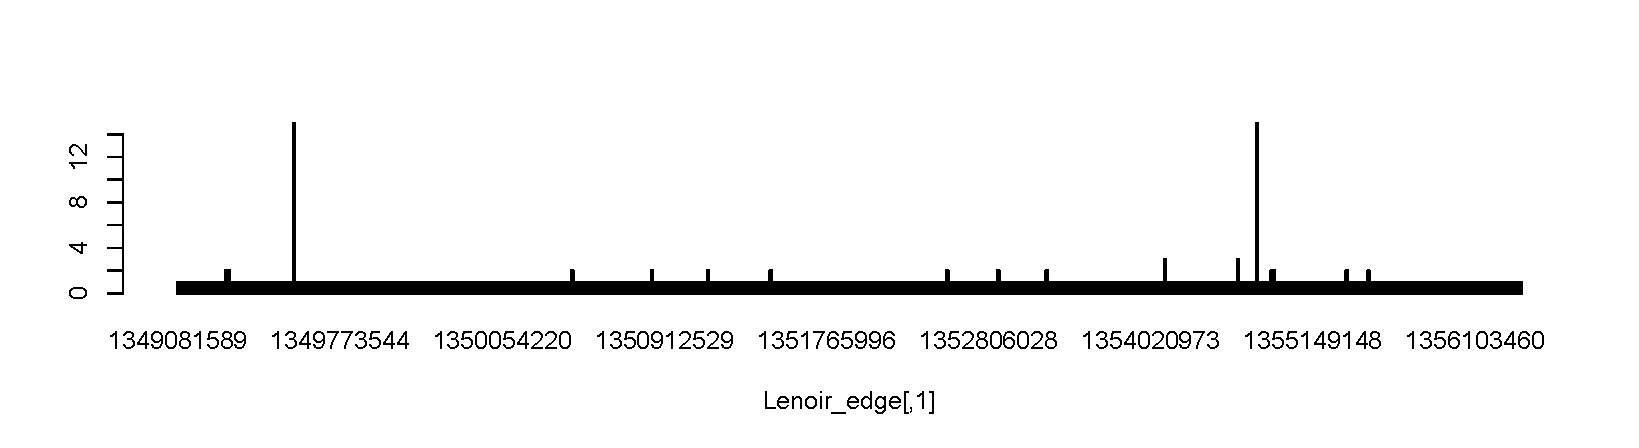
\includegraphics[width=1.1\textwidth]{LenoirEmails.pdf} 
	\caption{Frequency of Lenoir county emails from 2012-10-01 to 2012-12-31  }
	\label{fig:Emailplots32}
\end{figure}
\newpage
\subsection{Vance County}
\footnotesize
\footnotesize
\begin{table}[ht]
	\centering
	\begin{tabular}{ |c|ccc|c| } 
		\hline 
		\textbf{Period} &\textbf{Before Sandy} & \textbf{During Sandy} & \textbf{After Sandy} & \textbf{Overall} \\ 	\hline
		\textbf{\# emails}& 198& 18 & 55 & 271 \\ 
		\hline
	\end{tabular}
	\caption{ Summary of Vance county email data based on time period}
	\label{table:nullVance}
\end{table}
\normalsize
Before Sandy ranges from 2012-09-04 to 2012-10-21 (7 weeks), During Sandy ranges from 2012-10-22 to 2012-11-02 (2 weeks), and After Sandy ranges from 2012-11-03 to 2012-11-30  (4 weeks).
\footnotesize
\begin{figure}[ht]
	\centering
	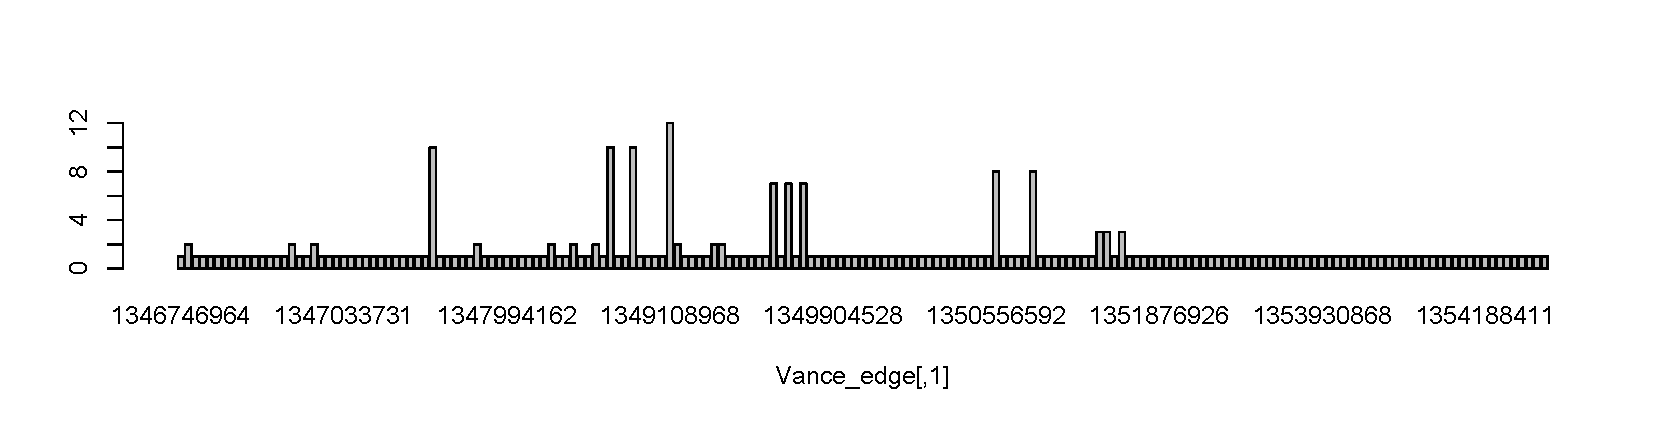
\includegraphics[width=1.1\textwidth]{VanceEmails.pdf} 
	\caption{Frequency of Vance county emails from 2012-09-04 to 2012-11-30  }
	\label{fig:Emailplots22}
\end{figure}
\bibliographystyle{apalike}
\bibliography{BominBib}

\end{document}